\chapter{Smart Grid Power Flow Status Monitoring}




\section{Time Synchronisation Protocols}

\subsection{Introduction}
Time Synchronisation protocols are used in order to synchronise the time of interconnected devices in need of synchronised time for various purposes. In the case of synchrophasor devices, the devices needs to be time synchronised in order for \acrshort{sg} \acrshort{wams} operators to get a correct overview of the system state.



The \acrshort{ptp} is included in the IEC standard

%\subsection{Synchrophasor data alignment attack}
Eq \ref{DMS} about DMS, and  eq \ref{DSM} about DSM.






\subsection{Synchrophasor Protocols}

\hl{The introduction of Synchrophasors in the} \acrlong{pg}, 

\subsubsection{Introduction}



As described in \cite{martin2011synchrophasor} and \cite{ali2016performance}, the \acrfull{pmu}, along with the \acrfull{pdc}, were introduced in the 1980s. The communication and data exchange from the PMU to the PDC was standardised by the introduction of the IEEE 1344 standard in 1995, which was established as the standard communication protocol for synchrophasor data exchange. According to \cite{appasani2018review}, the IEEE 1344 was revised in 2001 , before the introduction of the IEEE C37.118 in 2005. The  IEEE C37.118 protocol was derived from the IEEE 1344 standard, and has undergone a number of revisions, over the years.


In \cite{martin2013synchrophasor}, \citeauthor{martin2013synchrophasor}describes the history of the 
IEEE C37.118-series of satndards. The characterisitcs of the various generations, might be summarised as:
\begin{itemize}
    \item The IEEE C37.118-2005,
    \item The IEEE C37.118-2011
    \item The IEEE C37.118-2018
\end{itemize}




%Unlike the \acrlong{cpg}, the \acrlong{sg} enables bidirectional flow of power, by customers operating micro grids enabling customers to sell excessive power back to the network.








%\section{Historical}
%SCADA monitoring flaws -> PMU




%\section{PMUs}
%PMU
%-  Descripton of PMU
%- phasor
%- synchronised phasors
%- Communication with PDC

%\section{PDCs}
%PDC
%- Collecting synchronised phasors from PMU
%- Grouping synchronised phasors with same timestamp into Synchrophasor record
%- At deadline, transmitting Synchronaised phasors, received before deadline.
%- Improved security. 
%\section{Synchrophasors}
%Synchrophasors
%- overview
%- sync precision requirements:
 
%\section{Protocols used for monitoring}
%Protocols
%- Figure from PowerPoint
%- Concentrating on upper left side of figure.


%- capabilities of x.2011 x=synchrophasor protocol

%PTP
%Rationale for concentrating on PTP
%Descriptino of the protocol
%Time synchronisation via PTP
%PTP delay attack (types)


\section{Time Synchronisation}
In order to synchronise the samples received from the \acrshort{pmu}, the \acrshort{pdc}, as well as the \acrshort{pmu} devices producing the samples, precise timing adjustments is vital, in order to establish a precise and correct overview of system state. Incorrect synchronisation of measurements caused by erroneous timing information, will produice an equally wrong system state overview, as presented in the \acrshort{sg} \acrshort{wams}. \\ 


In order to be able to synchronise events in time, it is mandatory to adjust the clock of each participating actor, analogous to the classic pre-operational physical watch-synchronisation meetings in the physical domain. \\ 

The \acrshort{sg} time synchronisation requirements are, to say the least, a bit more demanding than a simultaneous press on a button. Several articles, of which \cite{appasani2018review} may serve as an example,  of by utilising a precise and reliable times source.  Given the distributed nature of the \acrshort{pmu} devices providing samples from locations distributed over a Wide Area Network, the \acrfull{gps} is the  time source selected. 

\subsection{Introduction}


The dependency on networking favors the usage of low-cost \acrshort{gnss} receivers for synchronising time between the growing number of \acrshort{pmu}s deployed at various locations, monitoring energy flow states of the highly distributed \acrshort{sg}. 



\subsubsection{The Importance of Time Synchronisation}

In \cite{dagle2019importance}, \citeauthor{dagle2019importance} states the following aspects as the benefits for Smart Grid operation, of ensuring correct time synchronisation:


\begin{itemize}
    \item  Situational Awareness and Wide-Area Monitoring
    \item  Real-Time Operations
    \item  Power System Planning 
    \item  Forensic Event Analysis
    
\end{itemize}

\subsubsection{Possible effects of Time Synchronisation errors}
Timing errors will, according to ,,, render the data introduced to the \acrshort{wams} system inadequate to enable \acrshort{sg} operatiors to get overview of the Energy supply state of the \acrshort{sg}.

In \Cite{martin2019impact}, \citeauthor{martin2019impact} lists a number of side-effects which could result form the absence of high-quality data material from the \acrshort{wams}.


\begin{enumerate}




    \item Data loss,
    \item Data corruption,
    \item Inaccurate representation of engineering quantities,
    \item Lack of precision,
    \item Incorrect measurement identification,
    \item Excessive or inconsistent latency.

\end{enumerate}

\subsubsection{Precision Time Protocol services}
The \acrfull{ptp} is a network-based time protocol, enabling the time difference between devices to be synchronised within a fraction (in the order of a few $\mu$s) of a second, satisfying the requirements of the \acrshort{sg}. 

\begin{figure}[ht]
    \centering
    \includegraphics[ width=\textwidth]{figures/PTP-timing-Diagram.png}
    \caption[Timing diagram for synchronization messages]{As presented in \cite[p. 51]{Eidson2006}: Timing diagram for synchronization messages.} 
    \label{fig:PTP-timing-Diagram}
\end{figure}  

\subsubsection{Description of PTP time synchronisation}



A device, being synchronised  by the \acrshort{ptp} protocol, reads its system time from a clock which is continuously synchronised by a network of one or more slave clocks, being periodically synchronised via various types of hybrid\footnote{Hybrid clocks are a master clock for some clocks, while being a slave clock for others.} clocks, ultimately synchronised with a grand master clock.


The time of the slave clock, is being adjusted according to the following process:


Following the message exchange visualised by \figureautorefname { } \ref{fig:PTP-timing-Diagram}, the Slave clock  uses the time offset $\theta$ from the Master clock time, calculated by Equation \ref{eq:offset}, in order to synchronise with the Master clock. 


\begin{equation}
t_1 = t_0 + \theta + d_1 \label{eq:t1}
\end{equation}


\begin{equation}
t_3 = t_2 - \theta + d_2
\end{equation}

\begin{equation}
d_1 = d_2 = d
\end{equation}

\textbf{Bla bla }Equation \ref{eq:t1}

\begin{equation}
%offset
\theta = \frac{(t_2 - t_1) + (t_4 - t_3)}{2} \label{eq:offset}
%\div 2    
\end{equation}
In order to be able to achieve the time difference required, the \acrshort{ptp}, as described by  \citeauthor{Eidson2006}, in \cite{Eidson2006}, is dependant on:

\begin{itemize}
    \item Timestamped network events, messages, which is  used for synchronisation.
    \item A method of timestamp transmission as required for synchronisation.
    \item Overcoming any timing impairments introduced by system components.
\end{itemize}




\subsection{Smart Grid Time Synchronisation}



\subsubsection{Introduction}


The \acrlong{sg} is dependant on precise Time Synchronisation, as a Time Synchronisation error of a few $\mu$-seconds may result in \acrshort{sg} instability. The time stamps produced by Synchrophasors, pinpointing the exact time of any system event, is vital in order to ensure precise and reliable system state information.
In the event of a system alert being triggered by erroneous system state Information, corrective actions by operators might have undesired effects. 

\subsubsection[Smart Grid Time Sync Precision Requirements]{Smart Grid Time Synchronisation Precision Requirements}

In order to ensure the time precision required for the \acrshort{sg}, the correct selection of time synchronisation mechanisms is vital. 




\begin{figure}%[ht]
    \centering
    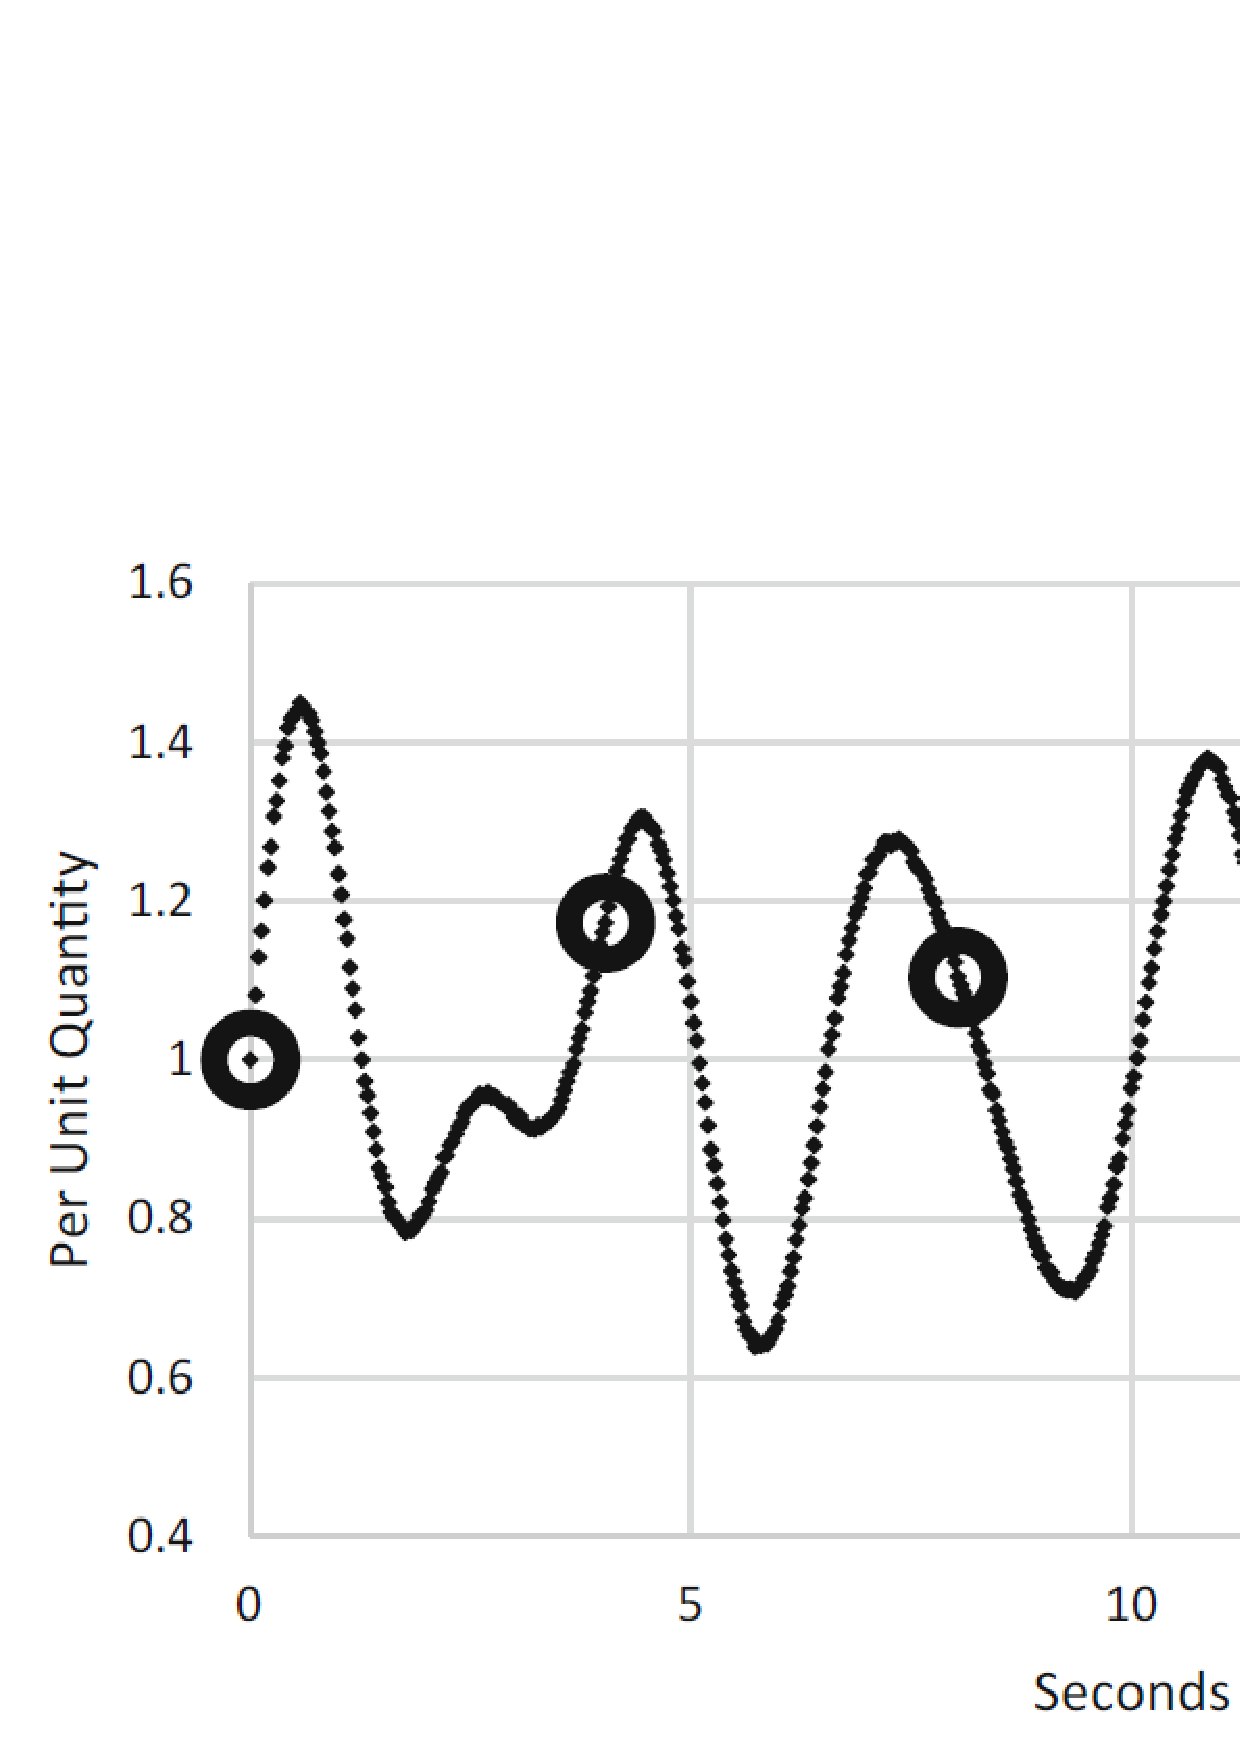
\includegraphics[ width=\textwidth]{figures/syncrophasors-vs-scada.png}
    \caption[Difference between Synchrophasor and SCADA measurements]{As presented in \cite[p. 3]{dagle2019importance}: Notional representation of the difference between synchrophasor and SCADA
measurement. Figure credit: \citeauthor{dagle2019importance}}.
    \label{fig:syncrophasors-vs-scada}
\end{figure}  

\subsection{Synchrophasor}
%\cite{ali2016wide}


%\Cite{rana2015exploring}



The \acrshort{pmu} is receiving values from sensors, on which it is able to calculate voltage level and phase angle of the energy flow. It is utilising a time-source to pinpoint measurements in time, producing synchrophasors, to be transmitted to the nearest \acrshort{pdc}. 

As described by \citeauthor{dagle2019importance} in \cite{dagle2019importance}, the data received from traditional \acrshort{scada} systems are time-stamped after arriving at the control station. The synchrophasors of the \acrshort{wams} on the other hand are, as described by \Citeauthor{ali2016wide} in \cite{ali2016wide}, being time-stamped in real-time before being transferred to the control system. The sampling rate of the \acrshort{pmu}, results in synchrophasor data enabling operators of the \acrshort{wams} to get real-time visualisation of critical elements, like the state of energy flow  of the \acrlong{sg}. The increased granularity of the measurement system allows for the detection of anomalies undetectable by traditional \acrshort{scada} systems, as illustrated by \figureautorefname { }\ref{fig:syncrophasors-vs-scada}. 

The increased sampling rate, of the synchrophasors of the \acrshort{wams} systems enables a more fine-grained view of energy distribution system state changes. However, in order for the \acrshort{wams} system to get the correct system state information, correct time stamps is critical. 
Therefore, the time-synchronisation mechanisms of the \acrshort{pmu} system is of critical importance. \\ 

\begin{figure}
    \centering
    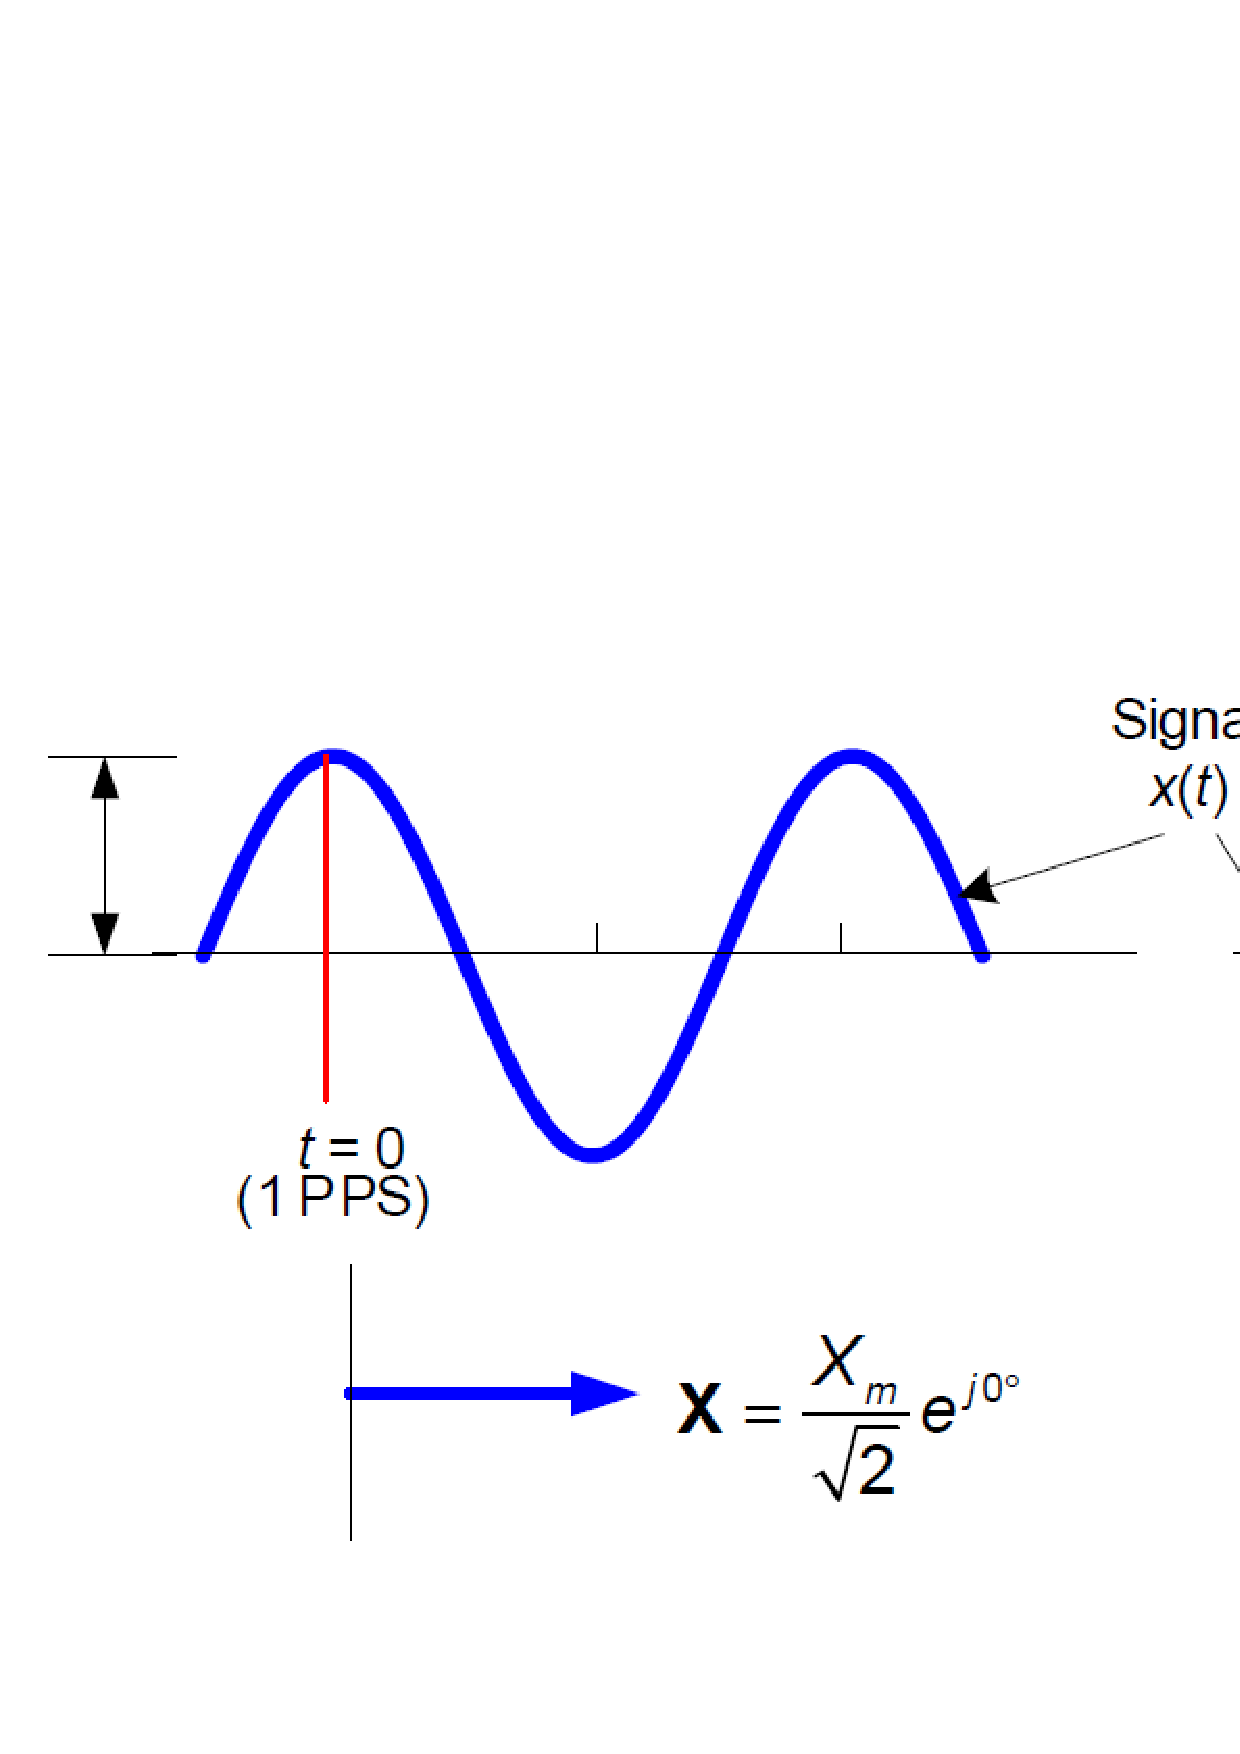
\includegraphics[ width=\textwidth]{figures/Synchrophasor-Definition.png}
    \caption[Convention for synchrophasor representation]{As presented in \Cite{schofield2018design}: Convention for synchrophasor representation.}.
    \label{fig:Synchrophasor-Definition}
\end{figure}  









\subsection{Time Synchronisation Protocols}
Time synchronisation protocols are controlling the synchronisation of time between various devices of the grid, like the PMUs, collecting phasor measurements from a definde number of measuring devices. Synchronised time is crucial in order to ensure each PMU is able to put the correct time stamp on each phasor measurement, before transmitting the resulting synchrophasor for each time stamp, to the destined PDC device. In the event one of the synchrophasors have an erroneous time stamp, an error affecting the integrity of the synchrophasor data is introduced. As described in \cite{moussa2016security}, \acrlong{ptp} synchronisation network
, as well as \acrlong{gnss} based synchronisation networks, are both capable of producing the precision required by the synchrophasor protocols, as opposed to the more common \acrfull{ntp} commonly used in ordinary computer networks. As my thesis covers \acrshort{ptp} time synchronisation only, my description of time synchronisation protocols is limited to the \acrfull{ptp}.

\subsubsection{Precision Time Protocol}

The \acrfull{ptp} was, \hl{as described in} \cite{alghamdi2021precision} ...

